\chapter{Continuous Integration}
\label{chap:continuous-integration}

The final phase of our project was to implement a continuous integration (CI) process for Synote. Only by deploying a new version of Synote and testing it can we be sure that a feature implementation is stable and functioning. However, a Synote experiment deployment has quite a few steps (\textbf{Figure \ref{fig:synote-ci-proc}}), which can take 15-30 minutes. In fact, it is completely infeasible to regularly repeat all the steps without hampering a developer's work. Since making a deployment takes  considerable time and is incredibly useful in continuous automated testing on remote deployments, we extended our project scope to implement Synote's first continuous integration process.

\section{Synote CI}
\label{sec:synote-ci}

A complete Synote CI process will deploy and test on the experiment deployment, followed by staging and finally production. Each stage will follow similar steps as Step 2 or the Experiment Deployment.

\begin{figure}[!hbt]
  	\centering
 	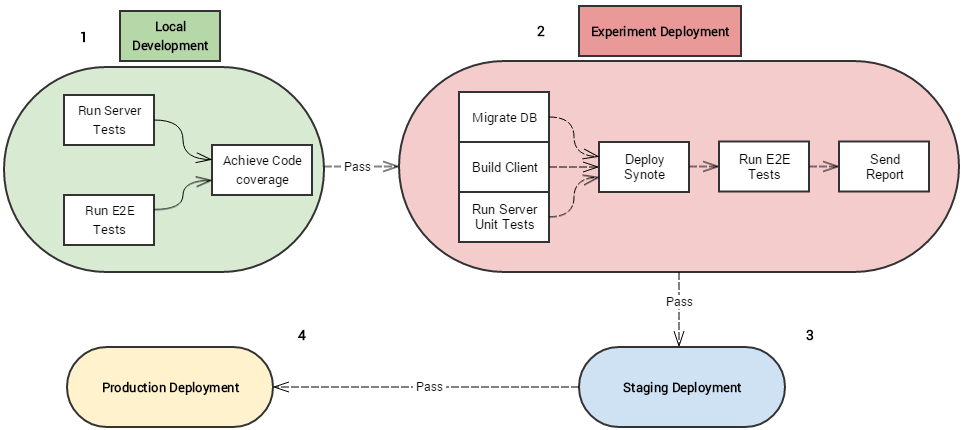
\includegraphics[width=\textwidth]{synote-ci.png}
  	\caption{Synote Continuous Integration Procedure}
 	\label{fig:synote-ci-proc}
\end{figure}

We focused on CI for the experiment deployment since we had access to it. In this chapter, we will elucidate the key steps necessary to configure a complete CI environment using Jenkins.\\

The key issues in this phase were -

\begin{itemize}

  \item Installing and configure Jenkins with SSL, restricted user access etc. (\textbf{Section \ref{subsec:setting-up-jenkins}})

  \item Synote is deployed as user \texttt{ubuntu}, however, Jenkins runs the build scripts as user \texttt{jenkins}. So, permissions for the deployment folders need to be rectified (\textbf{Listing \ref{lst:deployment-folder-permissions}}).

  \item \texttt{jenkins} needs to have access to the PM2 (a process manager) processes started by \texttt{ubuntu} (\textbf{Listing \ref{lst:jenkins-pm2-configuration}}).

  \item Running the E2E tests on a browser using a virtual display (\textbf{Section \ref{subsec:e2e-testing-on-remote}}).

\end{itemize}

\subsection{Setting up Jenkins}
\label{subsec:setting-up-jenkins}

We began by installing Jenkins on the experiment server (\textbf{Listing \ref{lst:install-jenkins}}). After monitoring the processes, we asked the client to upgrade the server to have 4GB RAM.

\begin{listing}[H]
\begin{minted}[xleftmargin=\parindent, linenos, breaklines, breakanywhere, bgcolor=lightgray, fontsize=\small]{bash}

# install Jenkins on Ubuntu (Synote Experiment Deployment)
wget -q -O - https://pkg.jenkins.io/debian/jenkins-ci.org.key | sudo apt-key add -
sudo sh -c 'echo deb http://pkg.jenkins.io/debian-stable binary/ > /etc/apt/sources.list.d/jenkins.list'
sudo apt-get update
sudo apt-get install jenkins

\end{minted}
\captionof{listing}{Install Jenkins}
\label{lst:install-jenkins}
\end{listing}

Then we added one admin account with complete Jenkins control, and one developer account with reduced control (e.g. cannot delete projects). Finally, we needed to run Jenkins behind a reverse proxy server (nginx) so that SSL encryption works properly and the domain reaches it (\textbf{Listing \ref{lst:make-jenkins-available}}).

\begin{listing}[H]
\begin{minted}[xleftmargin=\parindent, linenos, breaklines, breakanywhere, bgcolor=lightgray, fontsize=\small]{bash}

# nginx reverse proxy configuration for Jenkins

echo "upstream jenkins {
  server 127.0.0.1:8080 fail_timeout=0;
}

server {
  listen 80;
  server_name jenkins-cicd.synote.com; # dns for Synote CI
  return 301 https://$host$request_uri;
}

# ssl redirection

server {
  listen 443 ssl;
  server_name <synote_jenkins_ci_domain_name>;

  ssl_certificate <synote_ssl_certificate_location>;
  ssl_certificate_key <synote_ssl_private_key_location>;

  location / {
    proxy_set_header        Host $host:$server_port;
    proxy_set_header        X-Real-IP $remote_addr;
    proxy_set_header        X-Forwarded-For $proxy_add_x_forwarded_for;
    proxy_set_header        X-Forwarded-Proto $scheme;
    proxy_redirect http:// https://;
    proxy_pass              http://jenkins;
  }
}" > /etc/nginx/sites-available/jenkins

sudo service nginx restart

\end{minted}
\captionof{listing}{Make Jenkins server available on nginx}
\label{lst:make-jenkins-available}
\end{listing}

\subsection{Triggering Builds}
\label{subsec:triggering-builds}

\subsection{Pre-build Preparation}
\label{subsec:pre-build-preparation}

We first needed to give the ownership of \texttt{npm} modules to \texttt{ubuntu} (\textbf{Listing \ref{lst:npm-permission}}), so that we could install \texttt{bower}, which is needed to resolve the client app dependencies.

\begin{listing}[H]
\begin{minted}[xleftmargin=\parindent, linenos, breaklines, breakanywhere, bgcolor=lightgray, fontsize=\small]{bash}

# give permission to install global npm dependecies
sudo chown -R $USER:$GROUP ~/.npm
sudo chown -R $USER:$GROUP ~/.config

\end{minted}
\captionof{listing}{Global npm dependency permission}
\label{lst:npm-permission}
\end{listing}

\textbf{Listing \ref{lst:jenkins-build-script-variables}} is the different source-code locations on the experiment deployment that concerns the CI script. These will be necessary in the later listings.

\begin{listing}[H]
\begin{minted}[xleftmargin=\parindent, linenos, breaklines, breakanywhere, bgcolor=lightgray, fontsize=\small]{bash}

# the repos
SYNOTE_MAIN=/home/ubuntu/synote
SYNOTE_JENKINS=$WORKSPACE
E2E_JENKINS=$WORKSPACE/../gdp8-synote-e2e-testing
E2E_MAIN=/home/ubuntu/gdp8-synote-e2e-testing
REPORTS_WEBSITE_MAIN=$E2E_MAIN/reportsWebsite

\end{minted}
\captionof{listing}{Variables used during the Jenkins build script}
\label{lst:jenkins-build-script-variables}
\end{listing}

Then we give the permissions for the E2E testing and Synote deployment repo to a group that contains both \texttt{ubuntu} and \texttt{jenkins}. Now \texttt{jenkins} can make place new deployments of Synote.

\begin{listing}[H]
\begin{minted}[xleftmargin=\parindent, linenos, breaklines, breakanywhere, bgcolor=lightgray, fontsize=\small]{bash}

# create user group synote
sudo groupadd synote
sudo usermod -a -G synote jenkins
sudo usermod -a -G synote ubuntu

# permissions for e2e testing
sudo chown -R ubuntu: $E2E_MAIN
sudo chgrp -R synote $E2E_MAIN
sudo chmod -R 777 $E2E_MAIN

# permissions for synote
sudo chown -R ubuntu: $SYNOTE_MAIN
sudo chgrp -R synote $SYNOTE_MAIN
sudo chmod -R 777 $SYNOTE_MAIN

\end{minted}
\captionof{listing}{Deployment folder permissions}
\label{lst:deployment-folder-permissions}
\end{listing}

\begin{listing}[H]
\begin{minted}[xleftmargin=\parindent, linenos, breaklines, breakanywhere, bgcolor=lightgray, fontsize=\small]{bash}

# delete the .git folders from both repos
# since it creates files for ubuntu account only
rm -rf $SYNOTE_MAIN/.git
rm -rf $E2E_MAIN/.git

\end{minted}
\captionof{listing}{Deleting .git folders}
\label{lst:deleting-git-folders}
\end{listing}

\begin{listing}[H]
\begin{minted}[xleftmargin=\parindent, linenos, breaklines, breakanywhere, bgcolor=lightgray, fontsize=\small]{bash}

# Make locally installed programs available to jenkins
export PATH=${PATH}:/home/ubuntu/.nvm/v4.3.2/bin
export PM2_HOME="/home/ubuntu/.pm2"

# Make pm2 tasks started by 'ubuntu' available to 'jenkins'
sudo chmod 777 /home/ubuntu/.pm2/pub.sock
sudo chmod 777 /home/ubuntu/.pm2/rpc.sock

\end{minted}
\captionof{listing}{PM2 configuration for Jenkins}
\label{lst:jenkins-pm2-configuration}
\end{listing}

\subsection{Synote Build}
\label{subsec:synote-build}

\begin{listing}[H]
\begin{minted}[xleftmargin=\parindent, linenos, breaklines, breakanywhere, bgcolor=lightgray, fontsize=\small]{bash}

# building the server
cd $SYNOTE_JENKINS/backend
npm install

\end{minted}
\captionof{listing}{Building Synote server}
\label{lst:building-synote-server}
\end{listing}

\begin{listing}[H]
\begin{minted}[xleftmargin=\parindent, linenos, breaklines, breakanywhere, bgcolor=lightgray, fontsize=\small]{bash}

# building the client
cd $SYNOTE_JENKINS/frontend
npm install
bower install
grunt build:experiment

\end{minted}
\captionof{listing}{Building Synote client}
\label{lst:building-synote-client}
\end{listing}

\begin{listing}[H]
\begin{minted}[xleftmargin=\parindent, linenos, breaklines, breakanywhere, bgcolor=lightgray, fontsize=\small]{bash}

# replace the assets in /backend with the new frontend build
cp -RT $SYNOTE_JENKINS/frontend/dist/ $SYNOTE_JENKINS/backend/assets/

# Copy the synote repo from 'jenkins' to synote in 'ubuntu'
cp -RT $SYNOTE_JENKINS $SYNOTE_MAIN

\end{minted}
\captionof{listing}{Replace the current experiment deployment source}
\label{lst:replace current deployment source}
\end{listing}

\subsection{Automated Database Migration}
\label{subsec:automated-database-migration}

\begin{listing}[H]
\begin{minted}[xleftmargin=\parindent, linenos, breaklines, breakanywhere, bgcolor=lightgray, fontsize=\small]{bash}

# Run database migration
# Currently it's hardcoded to the latest migration but in the future,
# this should be decided on runtime depending on the database version
cd $SYNOTE/backend/db/migrate
mysql -u synote '-p<mysqlpass>' synote_server_experiment < procedures.sql # update procedures
mysql -u synote '-p<mysqlpass>' synote_server_experiment < v0.9.0-v0.10.0.sql # do migration

\end{minted}
\captionof{listing}{Automated DB Migration}
\label{lst:automated-db-migration}
\end{listing}

\subsection{Restarting the New Build}
\label{subsec:restarting-the-new-build}

\begin{listing}[H]
\begin{minted}[xleftmargin=\parindent, linenos, breaklines, breakanywhere, bgcolor=lightgray, fontsize=\small]{bash}

# always use pm2 app name to restart
pm2 restart synote_experiment

\end{minted}
\captionof{listing}{Restart experiment deployment}
\label{lst:restart-experiment-deployment}
\end{listing}

\subsection{E2E Testing on Remote}
\label{subsec:e2e-testing-on-remote}

\begin{listing}[H]
\begin{minted}[xleftmargin=\parindent, linenos, breaklines, breakanywhere, bgcolor=lightgray, fontsize=\small]{bash}

# cloning e2e repo
rm -rf $E2E_JENKINS

cd $SYNOTE_JENKINS/..
git clone git@bitbucket.org:sh3g12/gdp8-synote-e2e-testing.git

# copy over the content to 'ubuntu' e2e testing from 'jenkins'
cp -RT $E2E_JENKINS $E2E_MAIN

# install e2e main dependencies
cd $E2E_MAIN
npm install

\end{minted}
\captionof{listing}{Configure the latest E2E testing repository}
\label{lst:configure-latest-e2e-testing-repo}
\end{listing}

\begin{listing}[H]
\begin{minted}[xleftmargin=\parindent, linenos, breaklines, breakanywhere, bgcolor=lightgray, fontsize=\small]{bash}

# install reports website dependencies
cd $REPORTS_WEBSITE_MAIN
npm install

# restart the reporting server
pm2 restart reports_website

\end{minted}
\captionof{listing}{Deploy latest reporting website}
\label{lst:deploy-latest-reporting-website}
\end{listing}

\begin{listing}[H]
\begin{minted}[xleftmargin=\parindent, linenos, breaklines, breakanywhere, bgcolor=lightgray, fontsize=\small]{bash}

# start testing
cd $E2E_MAIN
npm test

\end{minted}
\captionof{listing}{Run E2E tests}
\label{lst:run-e2e-tests}
\end{listing}

\begin{listing}[H]
\begin{minted}[xleftmargin=\parindent, linenos, breaklines, breakanywhere, bgcolor=lightgray, fontsize=\small]{bash}

# install virtual display library
sudo apt-get install xvfb

# install Packages Required by browsers
sudo apt-get install x11-xkb-utils xfonts-100dpi xfonts-75dpi
sudo apt-get install xfonts-scalable xserver-xorg-core
sudo apt-get install dbus-x11

# install Browser
sudo apt-get install chromium-browser

\end{minted}
\captionof{listing}{Install virtual display library and browsers}
\label{lst:xvfb-browser-install}
\end{listing}

\begin{listing}[H]
\begin{minted}[xleftmargin=\parindent, linenos, breaklines, breakanywhere, bgcolor=lightgray, fontsize=\small]{bash}

# start the virtual display
echo "Xvfb :99" > $SYNOTE_JENKINS/xvfb_display.sh
pm2 start $SYNOTE_JENKINS/xvfb_display.sh

# start webdriver on the virtual display
echo "export DISPLAY=:99 && npm run start-manager" > $SYNOTE_JENKINS/depl.sh
pm2 start $SYNOTE_JENKINS/depl.sh

\end{minted}
\captionof{listing}{Start viertual display and webdriver as PM2 apps}
\label{lst:webdriver-pm2}
\end{listing}

\section{Usefulness of CI}
\label{sec:usefulness-of-ci}
